

\tikzset{every picture/.style={line width=0.75pt}} %set default line width to 0.75pt        

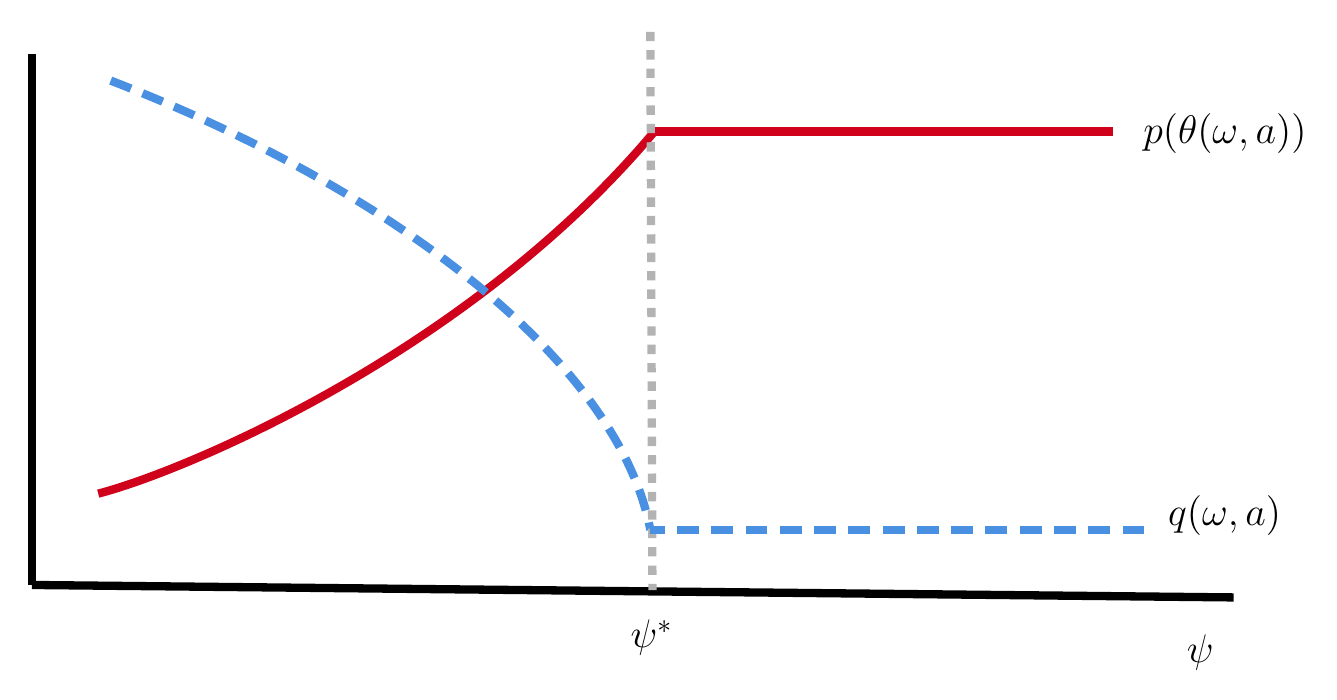
\begin{tikzpicture}[x=0.75pt,y=0.75pt,yscale=-1,xscale=1]
%uncomment if require: \path (0,326); %set diagram left start at 0, and has height of 326

%Straight Lines [id:da953931275515195] 
\draw [line width=3]    (36,273) -- (615,279) ;
%Straight Lines [id:da8868460884583611] 
\draw [line width=3]    (36,273) -- (36,17) ;
%Curve Lines [id:da06405175107936656] 
\draw [color={rgb, 255:red, 208; green, 2; blue, 27 }  ,draw opacity=1 ][line width=3]    (68,229) .. controls (112,217.5) and (248,159.5) .. (336,54.5) ;
%Straight Lines [id:da17850301166281368] 
\draw [color={rgb, 255:red, 208; green, 2; blue, 27 }  ,draw opacity=1 ][line width=3]    (336,54.5) -- (557,54.5) ;
%Curve Lines [id:da702887611986448] 
\draw [color={rgb, 255:red, 74; green, 144; blue, 226 }  ,draw opacity=1 ][line width=3]  [dash pattern={on 7.88pt off 4.5pt}]  (74,30) .. controls (215,84.5) and (319,167.5) .. (334,246.5) ;
%Straight Lines [id:da8828483808438534] 
\draw [color={rgb, 255:red, 179; green, 179; blue, 179 }  ,draw opacity=1 ][line width=3]  [dash pattern={on 3.38pt off 3.27pt}]  (334,6.5) -- (335,275.5) ;
%Straight Lines [id:da7866872337207746] 
\draw [color={rgb, 255:red, 74; green, 144; blue, 226 }  ,draw opacity=1 ][line width=3]  [dash pattern={on 7.88pt off 4.5pt}]  (572,246.5) -- (334,246.5) ;

% Text Node
\draw (591,295.4) node [anchor=north west][inner sep=0.75pt]  [font=\Large]  {$\psi $};
% Text Node
\draw (323,288.4) node [anchor=north west][inner sep=0.75pt]  [font=\Large]  {$\psi ^{*}$};
% Text Node
\draw (582,228.4) node [anchor=north west][inner sep=0.75pt]  [font=\Large]  {$q( \omega ,a)$};
% Text Node
\draw (570,44.4) node [anchor=north west][inner sep=0.75pt]  [font=\Large]  {$p( \theta ( \omega ,a))$};


\end{tikzpicture}